\chapter{Neutrino Beams}

Discussion of the design, realization and implementation of neutrino beams.  Proton sources, target materials, hadron interactions, horn focusing, produced particles, decay into neutrinos.  Also, discussion of beam simulation and flux estimation.  Neutrino and anti-neutrino running.

\section{Neutrinos from the Main Injector (NuMI Beam)}

History. Numi design and beam set up.  Hadron production, flux prediction.  Constraints from hadron production experiments.  Constraints from NuMI experiments: MINOS, Miner$\nu$a.  Energy mode.

\section{Booster Neutrino Beam}
\label{sec:bnb}

The Booster Neutrino Beame (BNB) is Fermilab's lower energy neutrino beam, and the primary beam of \MB, \uboone, and the Short Baseline Neutrino Program (see Chapter \ref{chp:sbn}).  The BNB is one of the most well understood, extensively studied neutrino beams in existence, and has been running since the \MB experiment and is expected to run until past 2020.

\subsection{Booster Neutrino Beam History}
The BNB was designed for, and by, the \MB collaboration.  \MB was a Cherenkov style detector, searching for electron neutrino appearance.  Because the primary background for \MB was photons from neutral pion production in the detector, which come from higher energy neutrinos, the BNB flux was designed to suppress neutrinos with energy above $\approx$ 1 GeV.

The origin of the BNB is 8 GeV protons (8.89 GeV/c momentum) from Fermilab's Booster complex.  These protons are transported to a Beryllium target, encased in a magnetic focusing horn.  The protons collide with the Be and produce hadrons within the target, which are focused into the forward direction by the focusing horn.  The hadrons enter a decay pipe of 50 meters, where they decay in flight into lighter particles including neutrinos.  At the end of the decay pipe is a beam stop to prevent all particles (except neutrinos) from proceeding.  A schematic of the proton entry, horn location, decay pipe and beam stop are shown in Figure~\ref{fig:mb_target_schematic}.

The primary source of the neutrinos in the BNB is from decay in flight pions, though there is significant contamination from kaon decay and muon decay (where the muons are also the product of pion decay).  The kaons and muons also produce a contamination of electron neutrinos in the primarily muon neutrino beam, and this flux of electron neutrinos is the primary background in the Short Baseline Neutrino Program's \nue appearance anaylsis.

\begin{figure}[tb]
  \centering
  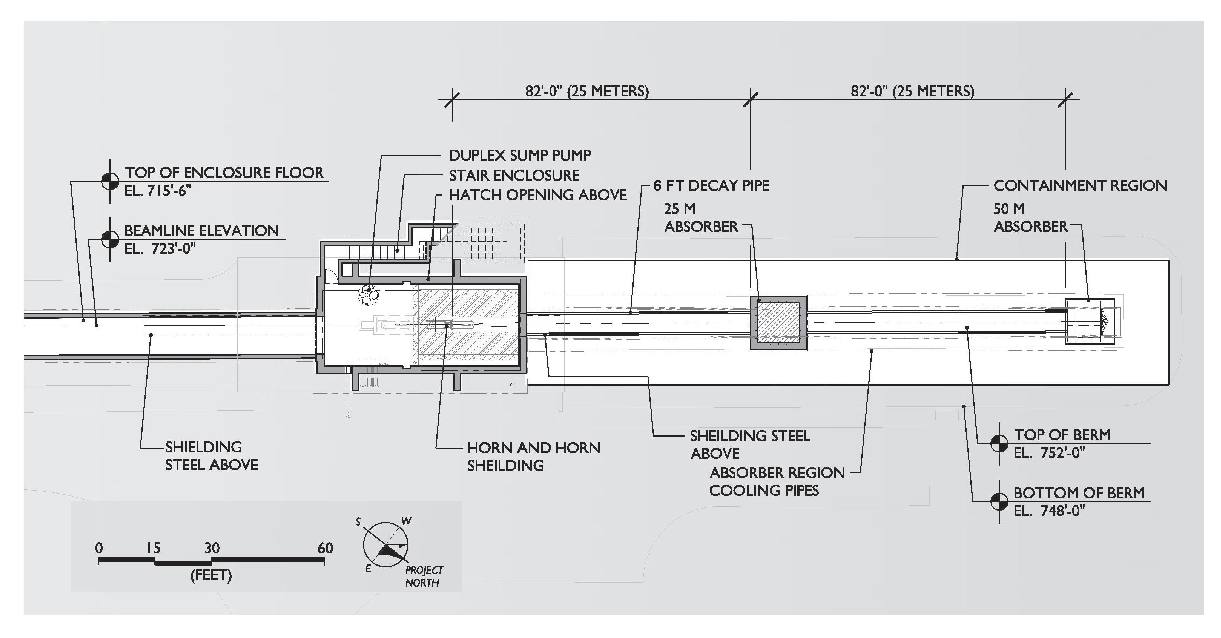
\includegraphics[width=\textwidth]{beams_figures/mb_target_schematic}
  \caption{The Booster Beam target hall and decay pipe.  Protons enter from the left, and hadrons decay in the decay pipe for up to 50m before the beam stop.  \MB, \uboone, and the other SBN experiments are to the right. Figure from \cite{AguilarArevalo:2008yp}}
  \label{fig:mb_target_schematic}
\end{figure}

The estimation of the flux, by neutrino type and by originating particle, at the \MB location can be seen in Figure~\ref{fig:mb_flux_nu}.  This estimate of the flux is produced with a sophisticated Monte Carlo simulation, discussed in detail in \cite{AguilarArevalo:2008yp}.  However, the general procedure is:

\begin{enumerate}

\item{Define the beamline geometry, including the shape, location, and composition of the components of the BNB.  This includes the target, magnetic horn, decay pipe and beam stop as well as the other minor parts.  The simulation attempts to capture the reality of the beam construction as closely as possible.  A graphical representation of the magnetic focusing horn can be seen in Figure~\ref{fig:mbhorn}.}

\item{Generate protons in the simulation that match the expected protons from the beam, accounting for the optical effects of the beam upstream of the target.}

\item{Simulate the interaction of protons in the target and surrounding material.  Substantial effort was made by the \MB collaboration to constrain this step of the simulation, as it is the primary source of systematic uncertainties in the beam model.  Dedicated experiments, such as HARP \cite{Catanesi:2007ab} and BNL E910 \cite{Chemakin:2007aa}, are used to constrain pion production and improve the flux prediction, as the uncertainties in pion production dominate the flux uncertainties.}

\item{Propagate particles from the primary interactions using GEANT\cite{Agostinelli:2002hh} to account for energy loss and interactions that change the kinematics of the particles above.  This also includes accounting for the focusing effects of the magnetic horn.}

\item{Identify particles that result in neutrinos at the detector, accounting for branching ratios and kinematic distributions properly.  Statistical boosting techniques are also used, since the solid angle subtended by the neutrino detector is small in the lab frame of the decaying particles.}

\end{enumerate}

\begin{figure}[tb]
  \centering
  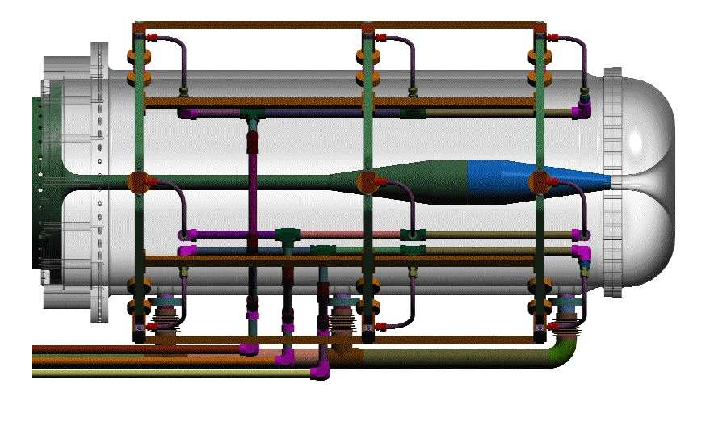
\includegraphics[width=\textwidth]{beams_figures/mbhorn}
  \caption{The Booster Beam horn and focusing magnet.  Figure from \cite{AguilarArevalo:2008yp}}
  \label{fig:mbhorn}
\end{figure}

\begin{figure}[tb]
  \centering

    \begin{subfigure}[t]{0.5\textwidth}
        \centering
        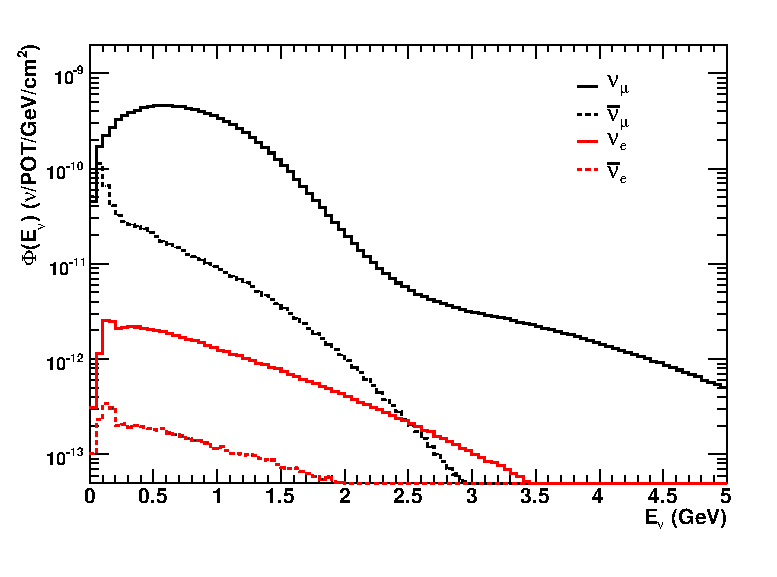
\includegraphics[height=2in]{beams_figures/mb_flux_nu}
    \end{subfigure}%
    ~ 
    \begin{subfigure}[t]{0.5\textwidth}
        \centering
        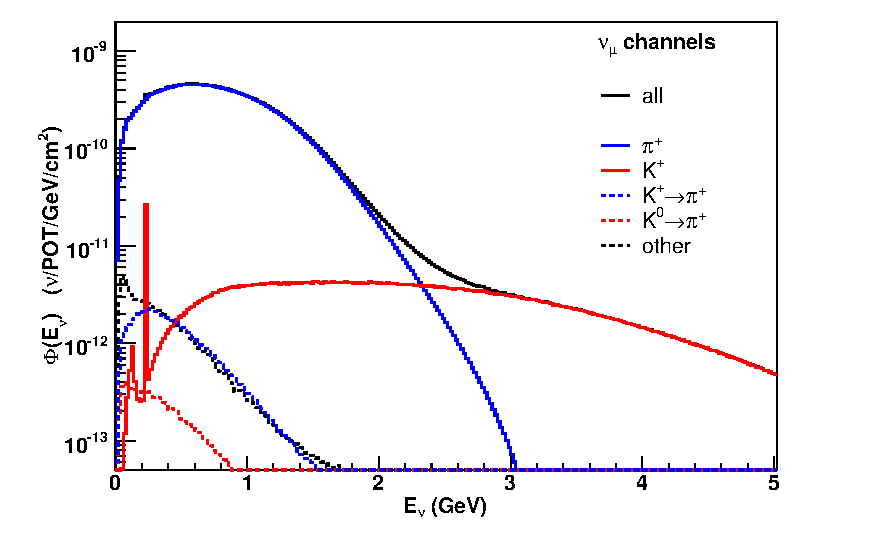
\includegraphics[height=2in]{beams_figures/mb_flux_by_type_nu}
    \end{subfigure}
  \caption{(Left) Total predicted flux at the MiniBooNE detector by neutrino species with horn in neutrino mode. (Right) Muon neutrino flux by type of original particle. Figure from  \cite{AguilarArevalo:2008yp}}
  \label{fig:mb_flux_nu}
\end{figure}

The work covered in this document does not use the \MB detector at all, however it does leverage the \MB flux calculation machinery to simulate the flux at multiple locations for the Short Baseline Neutrino Program.  In this light, the discussion of the systematic uncertainties of the flux prediction are left to Section~\ref{section:flux_uncert}.  However, Table~\ref{tab:mb_flux_uncert} is included here to showcase the precision at which \MB constrained the BNB, an accomplishment that future experiments are building upon.

\begin{table}[tb]
  \caption{Fractional flux uncertainties, by species of neutrino, from the \MB flux calculation.}
  \centering

  \begin{tabular}{l|rrrr}
  \hline
  \hline
  Source Of Uncertainty & \textbf{\numu} & \textbf{\numubar} & \textbf{\nue} & \textbf{\nuebar}  \\
  \hline
     Proton Delivery        &  2.0\% &  2.0\% &  2.0\% &  2.0\% \\
     Proton Optics          &  1.0\% &  1.0\% &  1.0\% &  1.0\% \\
     $\pi^+$ Production     & 14.7\% &  1.0\% &  9.3\% &  0.9\%\\
     $\pi^-$ Production     &  0.0\% & 16.5\% &  0.0\% &  3.5\% \\
     $K^+$ Production       &  0.9\% &  0.2\% & 11.5\% &  0.3\% \\
     $K^-$ Production       &  0.0\% &  0.2\% &  2.1\% & 17.6\% \\
     Horn Field             &  2.2\% &  3.3\% &  0.6\% &  0.8\% \\
     Nucleon Cross Sections &  2.8\% &  5.7\% &  3.3\% &  5.6\% \\
     Pion Cross Sections    &  1.2\% &  1.2\% &  0.8\% &  0.7\% \\
  \hline

  \hline
  \end{tabular}
  \label{tab:mb_flux_uncert}
\end{table}


\subsection{Future upgrades}
